\begin{GreyBox}
    \vskip-1cm
    \begin{block}{\GHead{Results}}

        \begin{center}
            \vskip-1cm
            \includegraphics[width=25cm,height=15cm]{img/Daily_TOPPs}
        \end{center}
        \vspace{1.5cm}
        \begin{flushright}
            %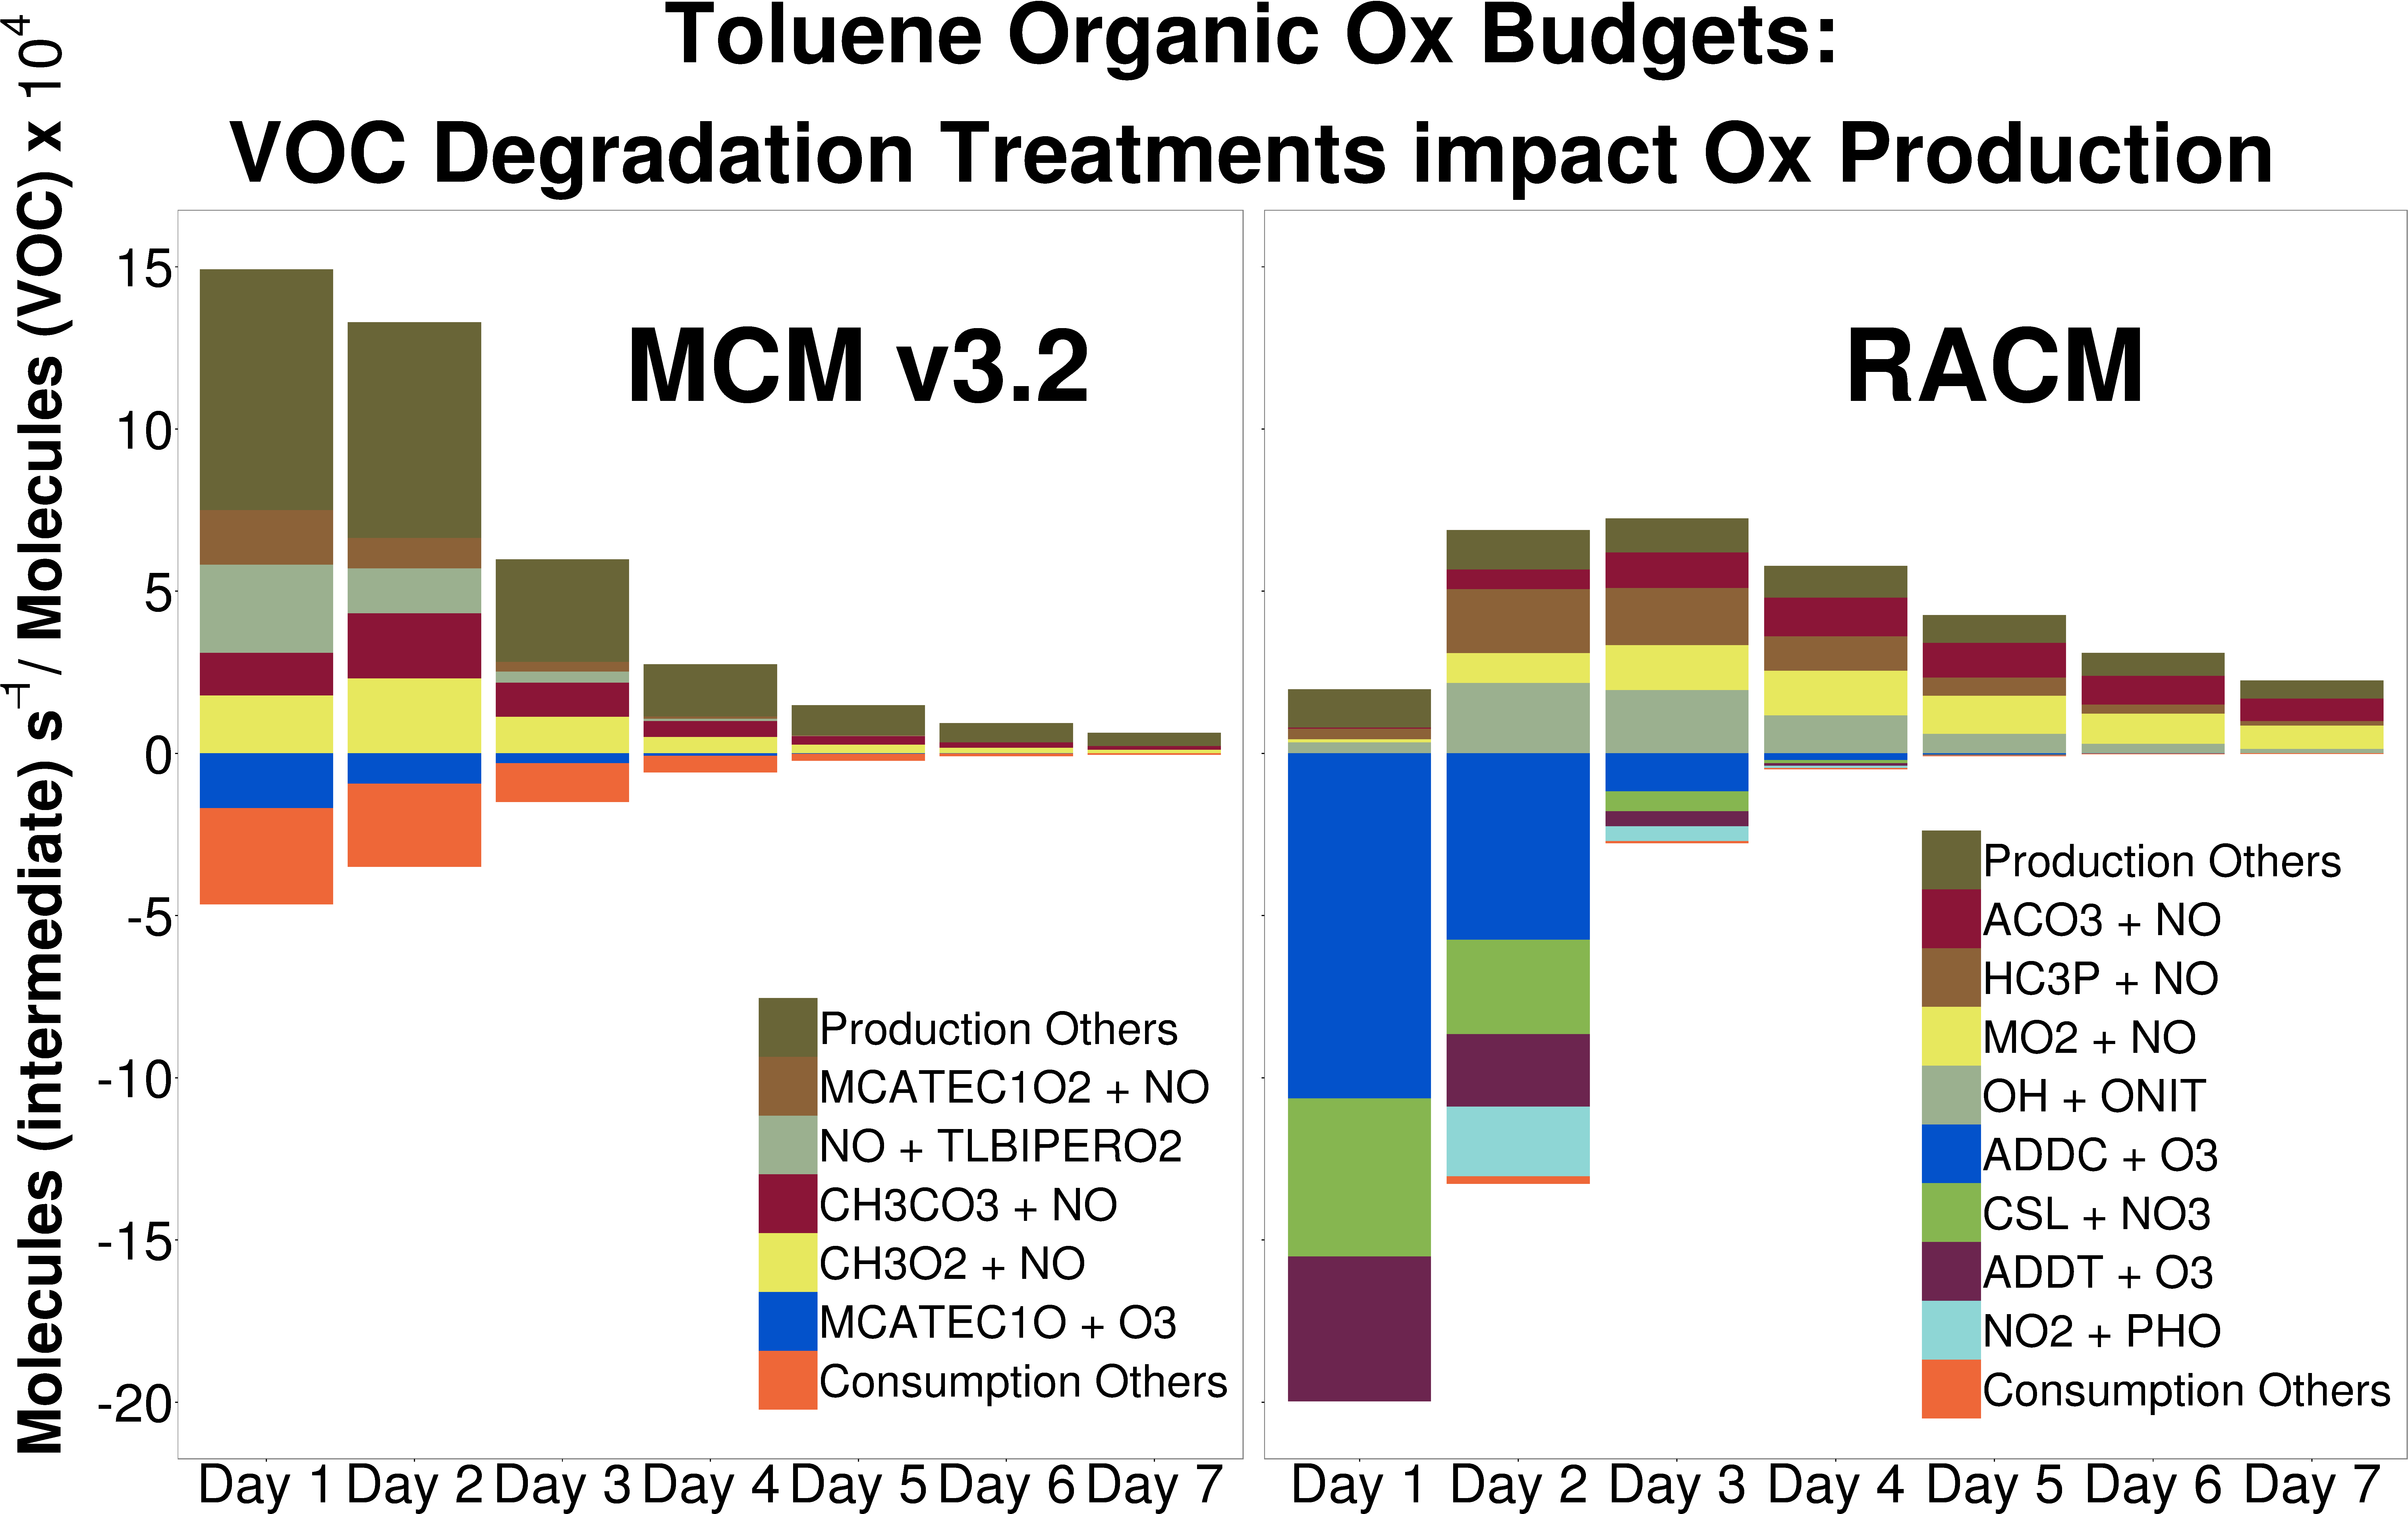
\includegraphics{img/TOL_MCM_RACM_Ox_intermediates}
        \end{flushright}
        \vspace{1.5cm}
        \begin{flushleft}
            %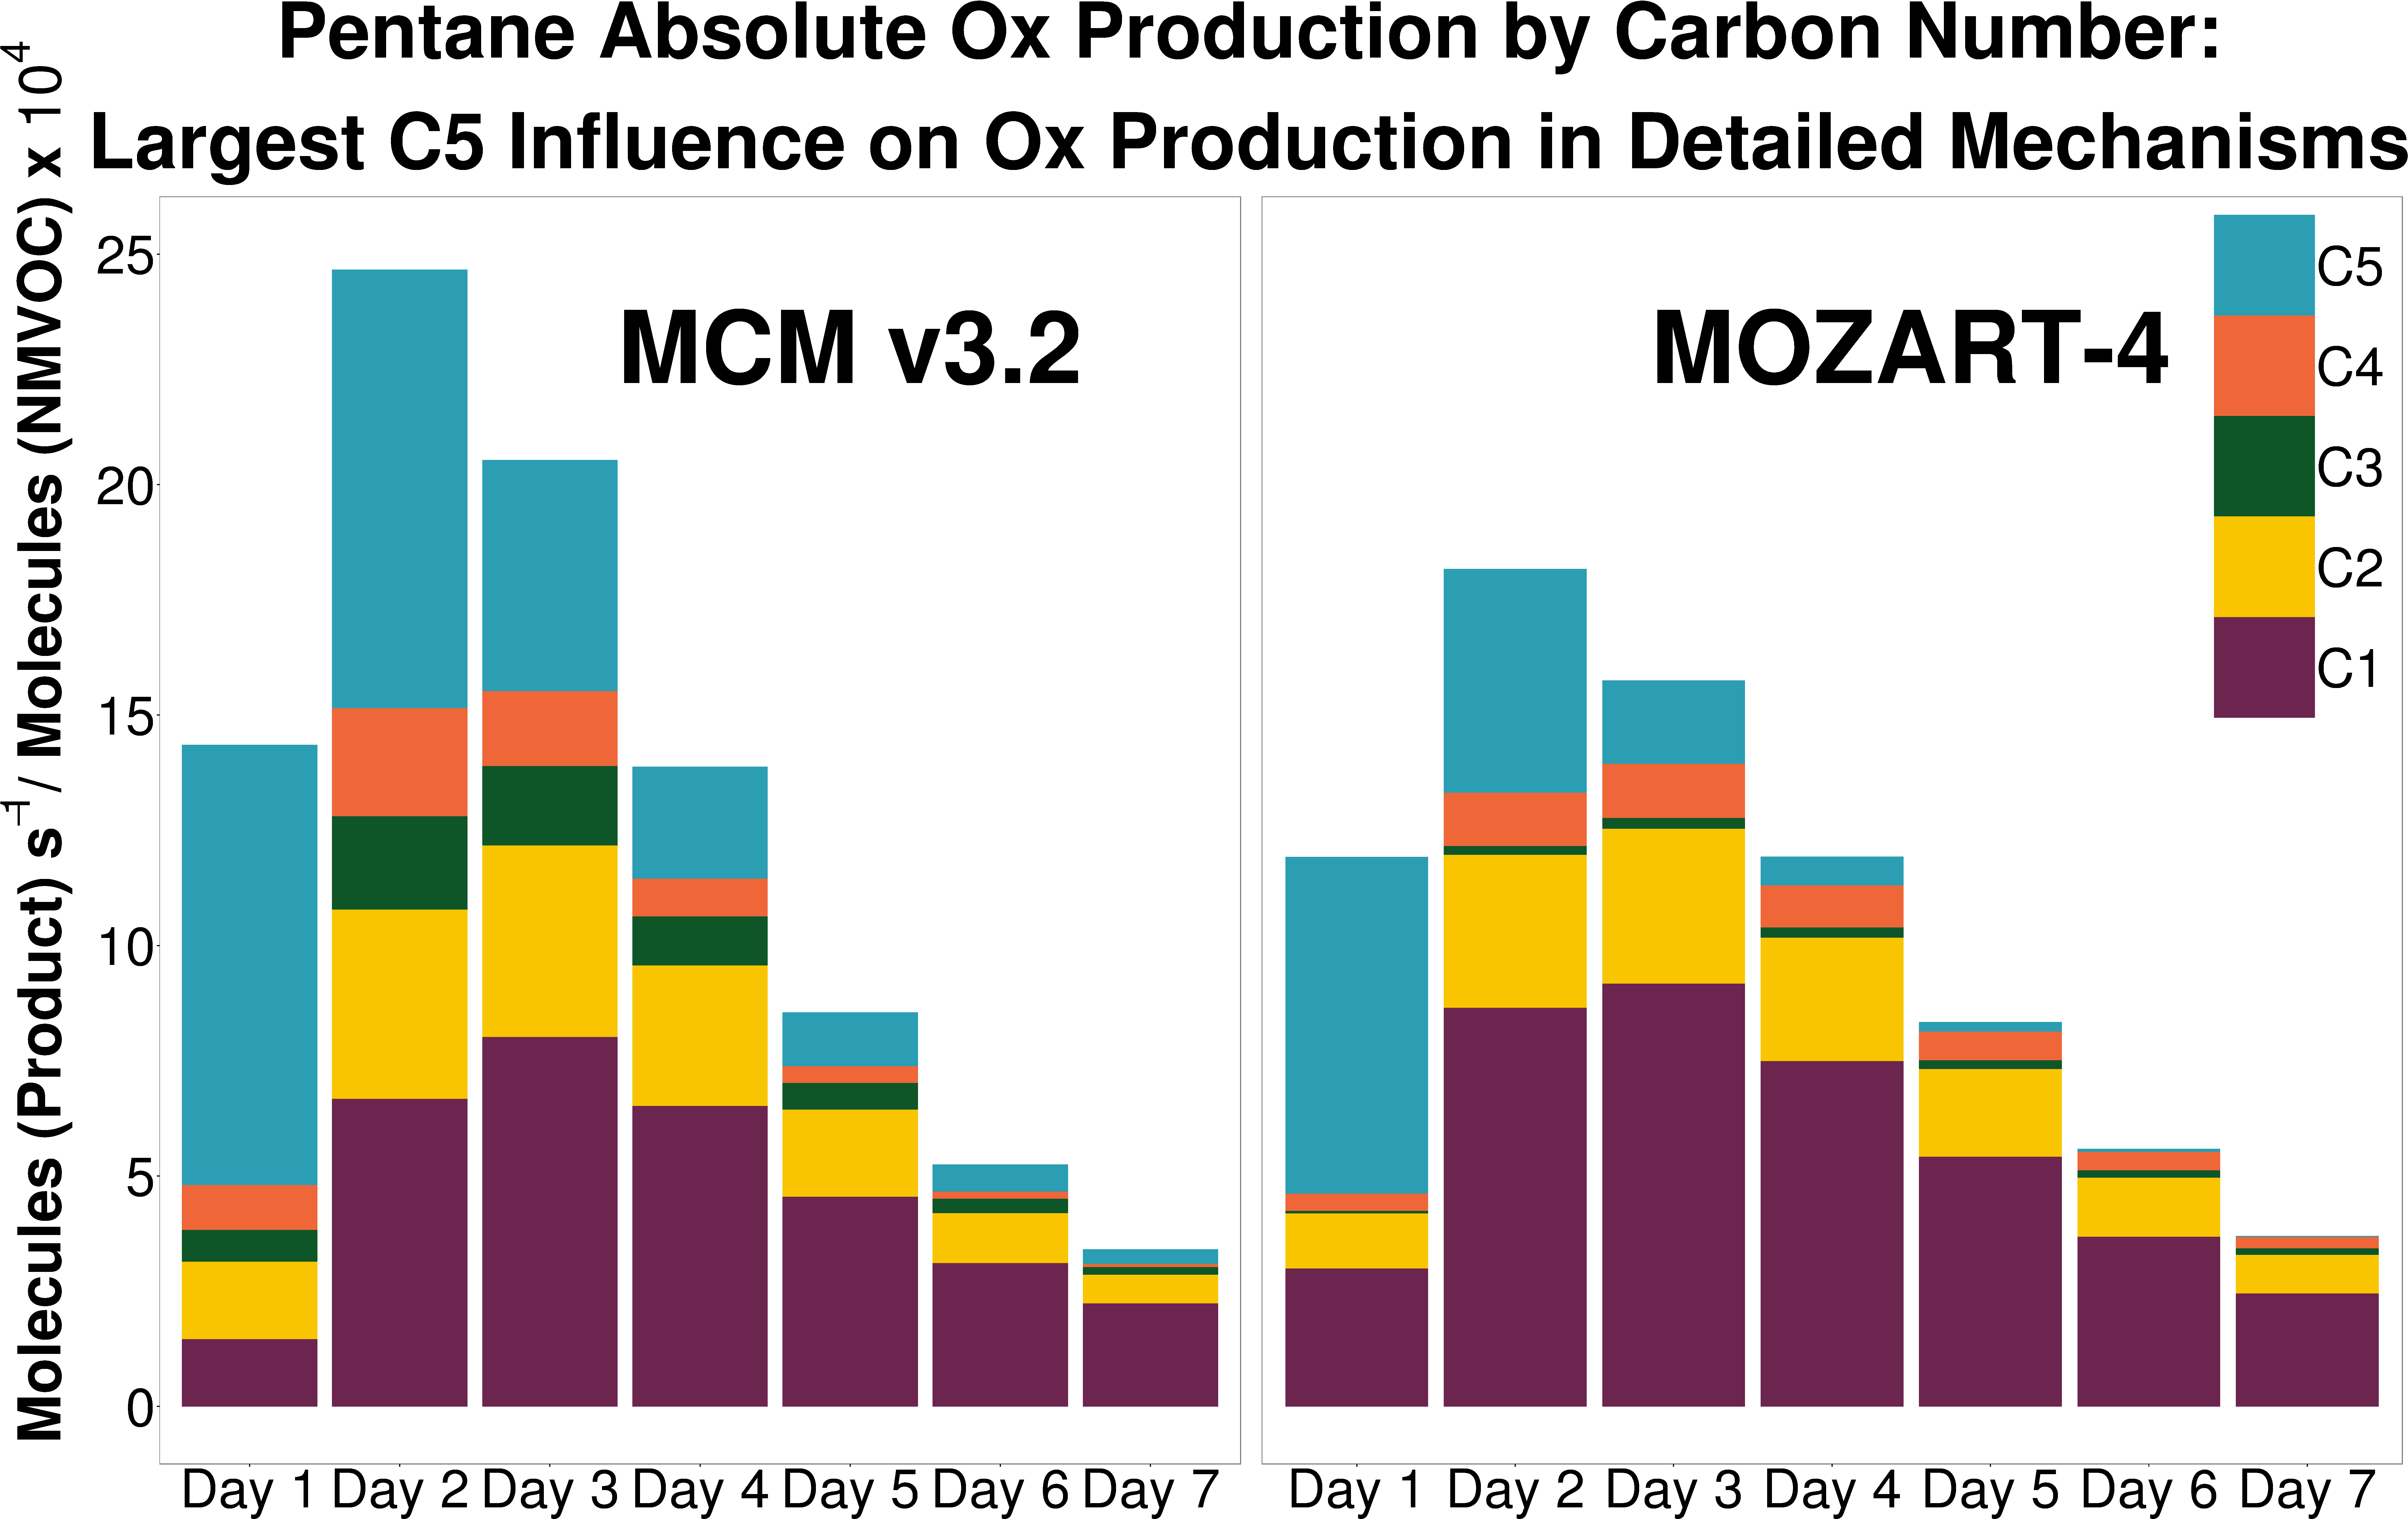
\includegraphics{img/pentane_carbon_breakdown}
        \end{flushleft} 
%        \tikzstyle{TOPP_box} = [draw=TitleBlue, rectangle, rounded corners, text width = 8.5cm, line width = 0.7mm]
%        \tikzstyle{aromatic_box} = [draw=TitleBlue, rectangle, rounded corners, text width = 12cm, line width = 0.7mm]
%        \tikzstyle{explanation} = [draw=TitleBlue, rectangle, rounded corners, text width = 7.5cm, line width = 0.7mm]
%        \tikzstyle{carbon_box} = [draw=TitleBlue, rectangle, rounded corners, text width = 13.5cm, line width = 0.7mm]
%        \begin{tikzpicture}[thick, overlay]
%            \node (placement) {};
%            \node (dummy_tol_TOPP) [above = 38.0cm of placement] {};
%            \node [draw=TitleBlue, ellipse, line width = 2mm, minimum width = 3em] (tol_TOPP) [right = 23.6cm of dummy_tol_TOPP] {};
%            \node (dummy_RACM) [above = 32.3cm of placement] {};
%            \node (RACM) [right = 31.5cm of dummy_RACM] {};
%            \path [-triangle 45, line width = 2mm, fill = TitleBlue, draw = TitleBlue] (tol_TOPP) edge node {} (RACM);
%
%            \node (dummy_pen_TOPP) [above = 40.9cm of placement] {};
%            \node [draw=TitleBlue, ellipse, line width = 2mm, minimum width = 7.5em, minimum height = 3em, rotate = 90] (pen_TOPP) [right = 13.8cm of dummy_pen_TOPP] {};
%            \node (dummy_left) [left of = pen_TOPP] {};
%            \node [coordinate] (left_TOPP) [left = 2.0cm of dummy_left] {};
%            \node [coordinate] (out_of_img) [left = 7mm of left_TOPP] {};
%            \node [coordinate] (left_most) [left = 9cm of out_of_img] {};
%            \node [coordinate] (dummy_c) [right = 1mm of left_most] {};
%            \node (pen_carbon) [below = 30.0cm of dummy_c] {};
%            \path [line width = 2mm, draw = TitleBlue] (pen_TOPP)  -- (left_TOPP);
%            \path [line width = 2mm, draw = TitleBlue] (out_of_img)  -- (left_most);
%            \path [-triangle 45, line width = 2mm, fill = TitleBlue, draw = TitleBlue] (dummy_c)  -- (pen_carbon);
%
%            \node (dummy_TOPP_box) [above = 6.0cm of tol_TOPP] {};
%            \node [TOPP_box] (TOPP_box) [right = 11.4cm of dummy_TOPP_box] {\begin{spacing}{1}\scriptsize{In general, the reduced mechanisms produce lower amounts of \ce{O_x}. The slower-reacting pentane has maximum \ce{O_x} production on day 2. This is reproduced to some extent by the mechanisms. Toluene profiles have a large spread throughout due to the varying representations of aromatic chemistry, which is not fully understood.}\end{spacing}};
%            
%            \node (dummy_aromatic_box) [below = 6.0cm of dummy_RACM] {};
%            \node [aromatic_box] (aromatic_box) [right = 2.5cm of dummy_aromatic_box] {\begin{spacing}{1}\scriptsize{RACM chemistry during the first 2 days results in net \ce{O_x} consumption, in contrast to the MCM v3.2 chemistry. This is due to \ce{O3} preferentially reacting with the mechanism species ADDC (OH-cresol adduct). This reaction is included in RACM on the basis of chamber data and its inclusion gave better cresol yields. This reaction is not included in any other mechanism and was removed in the updated RACM2 chemistry.}\end{spacing}};
%
%            \node (dummy_explanation) [below = 9.5cm of dummy_RACM] {};
%            \node [explanation] (explanation) [right = 19.0cm of dummy_explanation] {\begin{spacing}{0.65}\scriptsize{Overall budgets partitioned by individual reactions and each reaction has a different colour.}\end{spacing}};
%
%            \node (dummy_carbon_box) [below = 6cm of pen_carbon] {};
%            \node [carbon_box] (carbon_box) [right = 30cm of dummy_carbon_box] {\begin{spacing}{1}\scriptsize{The reduced mechanism MOZART-4 breaks down pentane quicker than the MCM v3.2. There is more influence from C5-products in the MCM v3.2, whilst there is more impact of C2- and C1-products in MOZART-4. Hence, breaking down the VOC quicker is impacting the timing and maximal amount of \ce{O_x} that can be produced.}\end{spacing}};
%        \end{tikzpicture}
    \end{block}
\end{GreyBox}
